\chapter{Resultados e Conclusões}
Neste capítulo mostraremos e analisaremos os resultados das implementações e modelagens discutidas anteriormente. Além disso, também traremos nossas conclusões e considerações finais sobre o trabalho.

\section{Mulligan}
Para cada estado (i, j), a recompensa associada à ação Keep nas tabelas 4.2 e 4.4 e, à direita, o valor
calculado $\Sigma$ da soma de valores associada à ação \textit{Mulligan}. As recompensas em vermelho indicam estados que a política extraída é \textit{Mulligan}.

TABELAS

A política encontrada com a iteração de valor faz bastante sentido se levarmos em consideração a simplificação de limitar a informação das cartas na mão ao fato dela ser terreno ou não. Uma maneira de deixar a modelagem mais real seria levar em consideração o custo de mana dos cards não-terreno. Isso aumentaria enormemente a quantidade de estados possíveis (supondo que as cartas não-terreno do deck tenham custo de mana entre 1 e 5, uma mão com duas cartas teria $\sum\limits_{i=1}^{6}i = 21$ representações possíveis de estados ao invés de 3, como acontece com a modelagem que escolhemos), mas essa modelagem ainda estaria desconsiderando informações relevantes na decisão do mulligan, como por exemplo se as cartas na mão inicial se encaixam na estratégia definida pelo jogador para combater o deck adversário. De uma maneira geral, estamos satisfeitos com os resultados obtidos, uma vez que o agente consegue mitigar a aleatoriedade tomando decisões que aumentam suas chances de ter um jogo justo.

\section{Simulações do Jogo}
Após rodar os experimentos várias vezes e analisar os resultados, conseguimos descrever o comportamento do agente dentro do jogo como agressivo: já que escolhemos uma implementação que leva em consideração apenas o turno atual, o agente não leva em conta o ataque do oponente no turno seguinte, e portanto escolhe os atacantes sem pensar em quais de suas criaturas seriam boas bloqueadoras para impedir que o oponente estabeleça uma vantagem ou até mesmo ganhe o jogo. Os decks usados para os testes serão chamados Branco e Vermelho, pelas cores de suas cartas.

Rodamos 70 testes com as configurações possíveis de agente inteligente ou aleatório controlando cada um dos decks, e obtivemos os seguintes resultados:

\begin{itemize}
\item \textbf{Aleatório x Aleatório}

\begin{figure}[!ht]
    \centering
    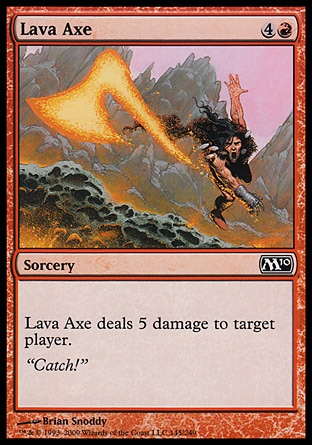
\includegraphics[width=0.3\textwidth]{picstcc/lavaaxe.jpg}
    \caption{A carta Lava Axe (Machado de Lava) pode ter qualquer jogador, incluindo seu controlador, como alvo}
    \label{lavaaxe}
\end{figure}

Para esta configuração, esperávamos que o deck Branco ganhasse mais do que o Vermelho, pois o deck Branco tem poucas cartas que possibilitam que o agente faça uma escolha \textit{muito} ruim, como destruir sua própria criatura. Já o deck Vermelho tem cartas como Lava Axe (\ref{lavaaxe}), que possibilitam que o jogador acerte a si mesmo, ou Volcanic Hammer, que pode ser usado para destruir suas próprias criaturas.

GRAFICO AQUI

Após as simulações, o deck Branco ganhou $71,8\%$ das vezes, superando um pouco as nossas expectativas, mas num nível aceitável.

\item \textbf{Aleatório x Inteligente}

Nesta configuração, esperávamos que os agentes inteligentes ganhassem praticamente todas as partidas.

GRAFICO AQUI

Jogamos com as duas configurações possíveis, e nas duas o agente com o algoritmo de busca se saiu
muito melhor que o oponente: $95,9\%$ quando no controle do deck Branco, e $97,2\%$ quando controlando o deck Vermelho. Novamente um resultado esperado, dado que o agente aleatório demora turnos para jogar seu primeiro terreno enquanto o agente inteligente joga terrenos sempre que possível, o que possibilita que jogue suas cartas muito antes.

\item \textbf{Inteligente x Inteligente}
Nesta configuração, esperávamos um desempenho um pouco melhor do deck Vermelho, uma vez que o comportamento do agente é agressivo graças a ele não olhar turnos a frente. Numa situação onde nenhum jogador está tentando preservar seu total de pontos de vida, quem tiver acesso a cartas como Lava Axe irá se beneficiar mais.

GRÁFICO AQUI

O resultado obtido foi $76,5\%$ de vitórias para o agente com o deck vermelho, próximo do que esperávamos.

A versatilidade providenciada por cartas que infligem dano também permitiu jogadas engenhosas da parte do agente Vermelho, como por exemplo a seguinte sequência de ações: atacar com ``Nest Robber'' (2/1) prevendo (corretamente) que o oponente o bloqueará com ``Siege Mastodon'' (3/5), o que causa com que ``Nest Robber'' seja destruído em combate. Na segunda Fase Principal, então, complementar o dano no ``Siege Mastodon'' (no momento com 2 de dano marcado) inimigo com ``Volcanic Hammer'', causando um total de 5 de dano capaz de destruir a criatura. Como os dois agentes inteligentes decidem bloquear baseando-se nas mesmas regras, as previsões sempre são corretas nessa categoria de testes.

\end{itemize}

\section{Conclusões}
O jogador inteligente implementado apresentou resultados interessantes de jogo e, apesar de podermos facilmente prever seu comportamento, as habilidades demonstradas são bastante valiosas em um jogo de Magic.

Um jogador (humano) por exemplo, deve balancear ganhos a curto prazo e ganhos potenciais a longo prazo, portanto definir as melhores jogadas a curto prazo faz parte do conjunto de habilidades de um bom jogador. Além disso, o jogador médio tem uma curva considerável de aprendizado para conseguir fazê-lo, enquanto esta habilidade se mostrou, de certa forma, ``natural'' para uma inteligência artificial, pois o algoritmo de busca local cumpre um bom trabalho em examinar e memorizar todas as possibilidades para decidir entre elas.

\subsection{Escopo}
Quando começamos o trabalho pretendíamos adicionar ao estudo o tratamento da informação incompleta
(o que tornaria o problema parcialmente observável\footnote{Em inglês, POMDP - ``Partially Observable Markov Decision Process''}), além de alguma implementação de aprendizado por reforço. Apesar de ambos terem sido descartados por uma questão de tempo, adicionar aprendizado por Q-Learning seria o próximo passo do projeto, pois poderíamos implementá-lo utilizando a busca local como base para as ações. Assim, uma ação para o problema de Q-Learning seria equivalente a um caminho de ações do problema da busca, e o agente de aprendizado por reforço poderia comparar dentre uma série de caminhos aquele com o maior Q-Valor, determinado dinamicamente pelo algoritmo de aprendizado. Assim, decisões a longo prazo poderiam ser contempladas. No que se refere à implementação do jogo de Magic, seria interessante continuar expandindo o problema para que contemplasse mais aspectos do jogo. Como por exemplo, a introdução de ``Mágicas Instantˆaneas'', cartas equivalente aos Feitiços, mas diferindo em que podem ser jogadas em um conjunto maior de momentos, incluindo turnos dos oponentes. O conjunto de regras de Magic: the Gathering é extremamente complexo, mas também igualmente robusto, o que possibilita definir suas mecˆanicas muito bem em uma implementação do jogo.

\subsection{Apreciação e considerações finais}
Implementar o nosso próprio cliente fez com que trabalhássemos com orientação a objetos em um projeto grande, o que não havíamos feito muito durante as disciplinas da graduação. O cliente facilitou a implementação dos agentes, uma vez que tínhamos conhecimento total da plataforma, mas por outro lado impossibilitou que testássemos os agentes corretamente até que o jogo estivesse funcionando corretamente, o que acabou se mostrando mais trabalhoso que o esperado. Ainda assim, fazer o cliente funcionar (e os algoritmos de busca também) se provou bastante satisfatório. Além disso, modelar os problemas de inteligência artificial do zero solidificou nossos conhecimentos e interesse na área, principalmente ao impor uma das maiores dificuldades do projeto: decidir quais modelagens e estratégias de resolução adotar. Como escolhemos um tema de nosso interesse pessoal (mais precisamente, um hobby), tivemos uma boa motivação para conseguir resultados (e ainda estudamos melhor as próprias nuances do jogo), mas por outro lado provou-se um desafio pois coube a nós decidir métricas e avaliar resultados.

Dentre as disciplinas cursadas no Bacharelado em Ciência da Computação relevantes para o desenvolvimento do projeto, destacamos:
\begin{itemize}
\item MAC0435 - Inteligência Artificial
\item MAC0211/MAC0242 - Laboratório de Programação I/II
\item MAC0441 - Programação Orientada a Objetos
\item MAC0338 - Análise de Algoritmos
\end{itemize}
Agradecemos ao Professor Denis Deratani Mauá, que como supervisor ajudou inúmeras vezes a nortear o
trabalho.
